
\section{Method}

\begin{figure*}[h]
    \centering
    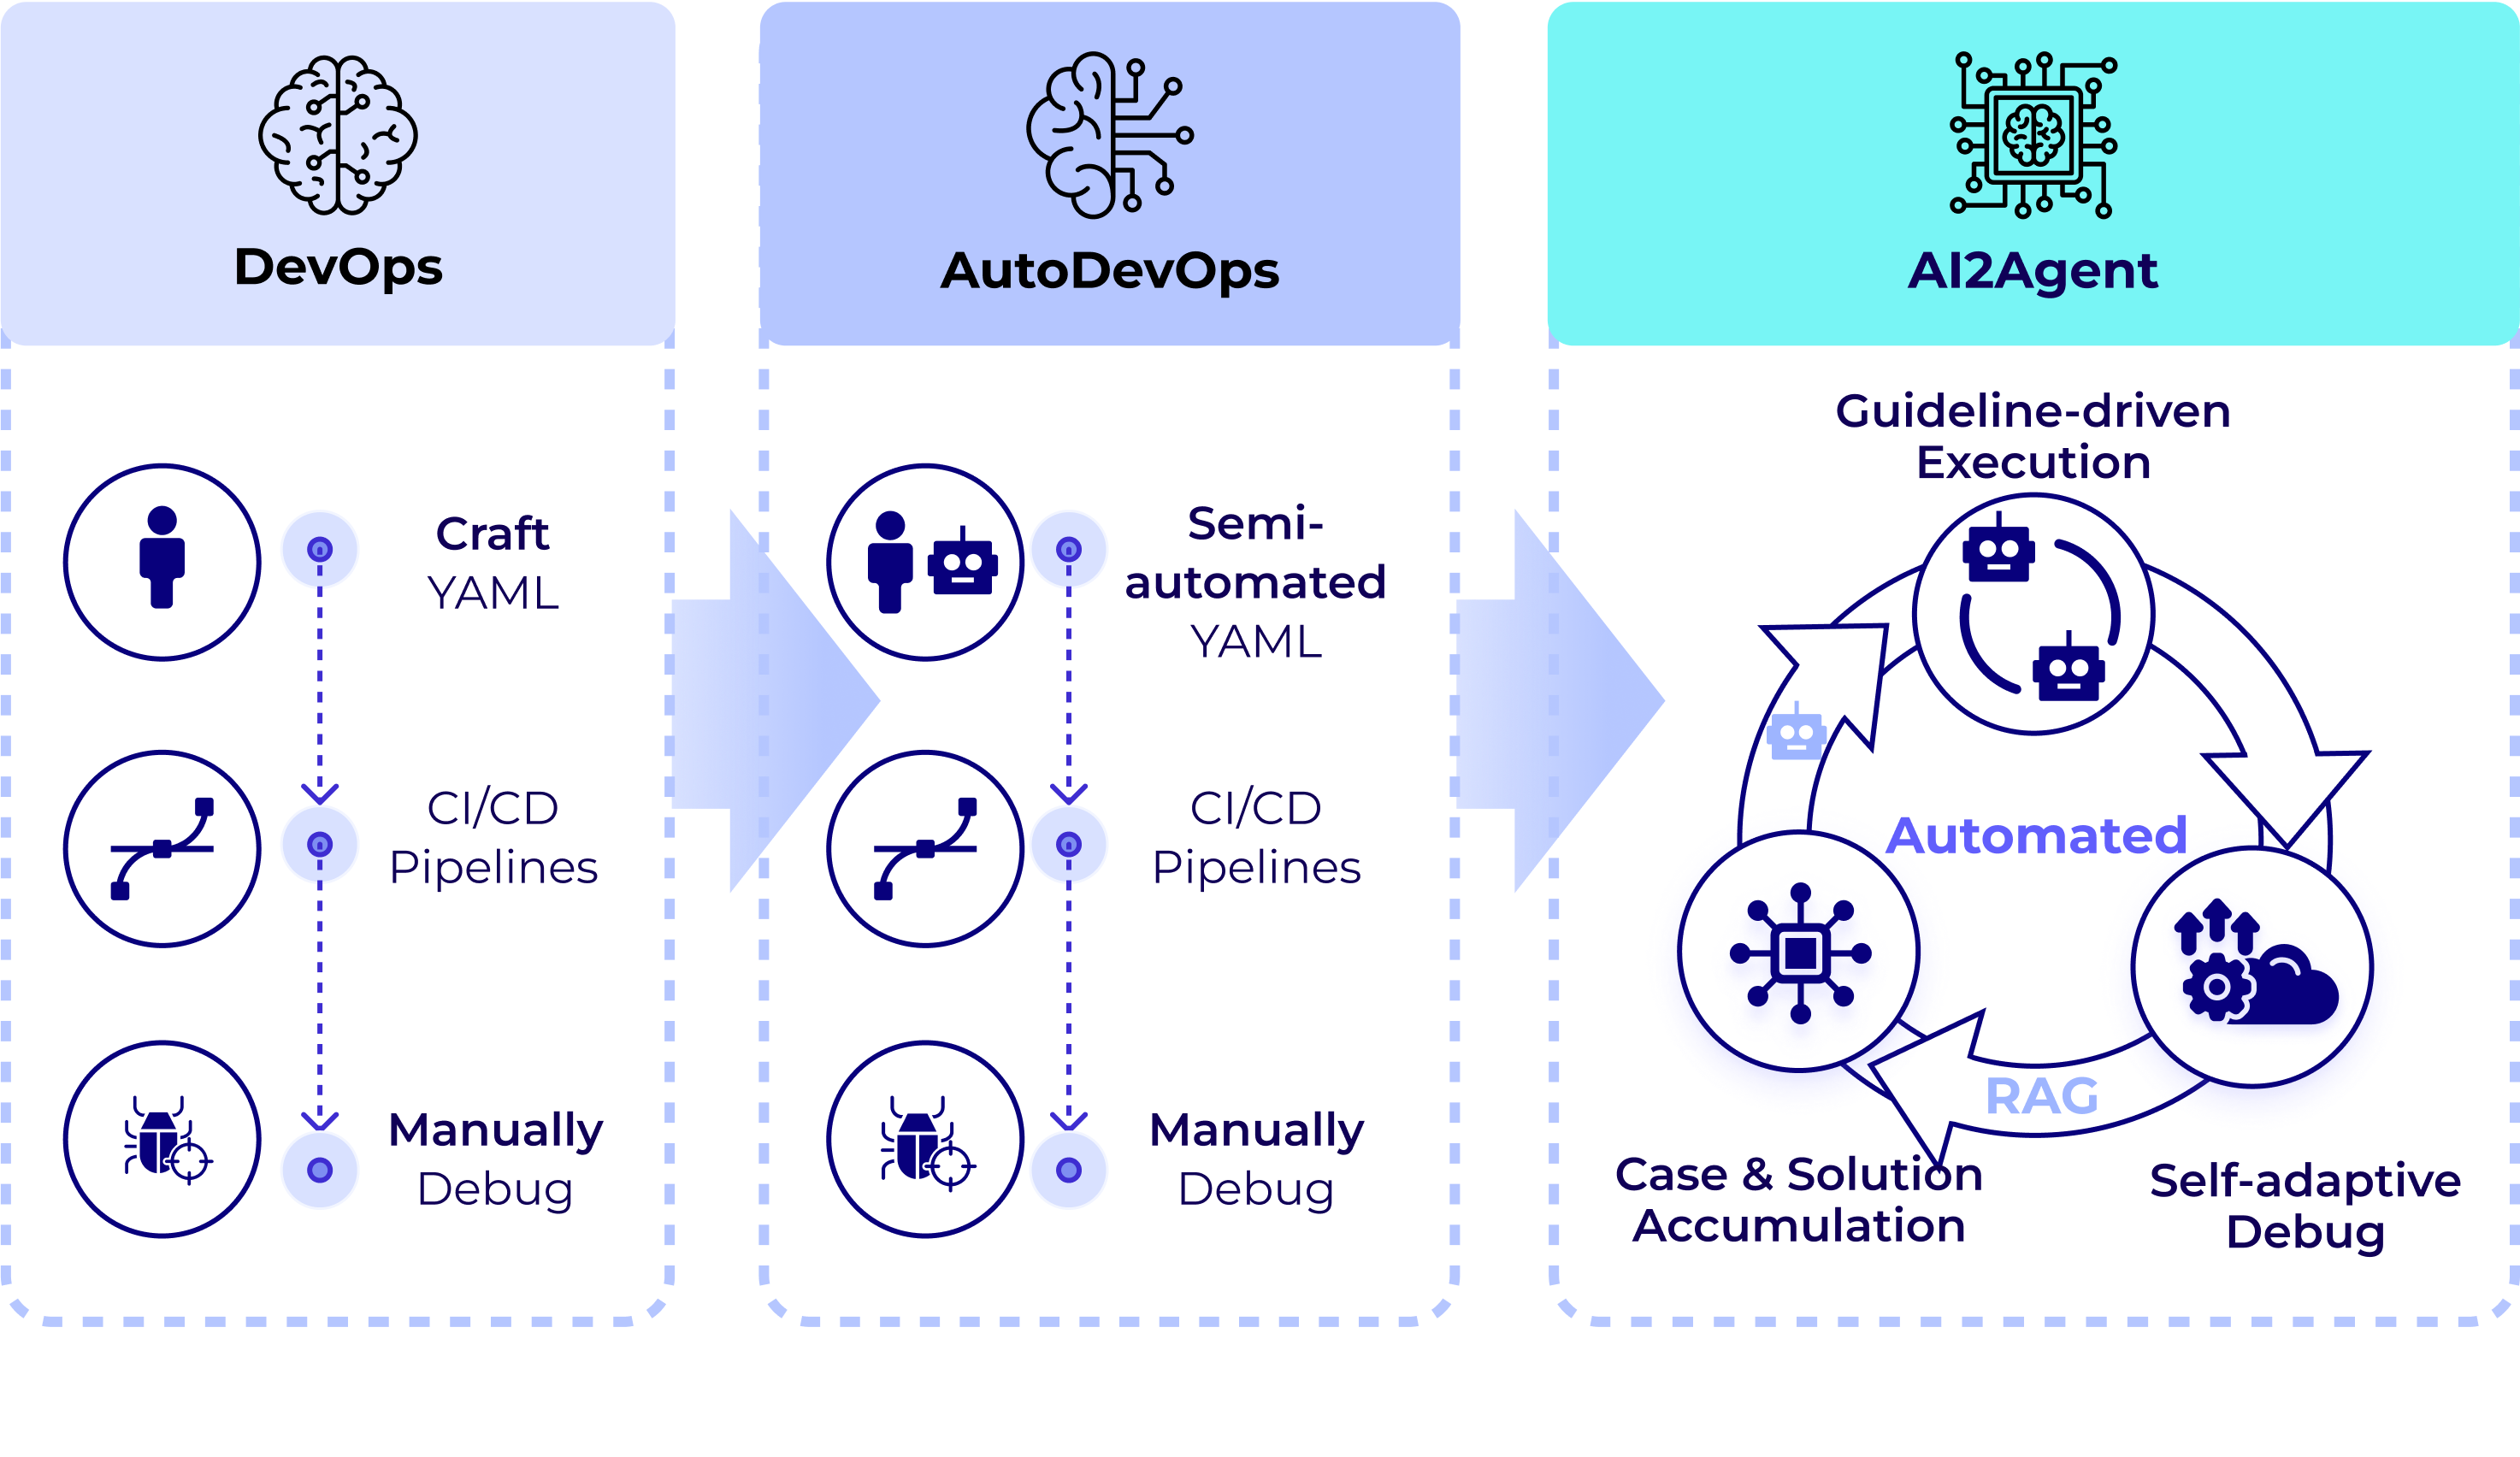
\includegraphics[scale=0.45]{imgs/comparison.png}
    \caption{Comparison of Paradigms. DevOps relies on manual YAML configuration and CI/CD workflows with manual debug. AutoDevOps offers semi-automated configuration but still requires human intervention. AI2Agent achieves end-to-end automated performance, including guideline-driven execution, self-adaptive debug, and case \& solution accumulation.}
    \label{fig:cmp_diagm}
\end{figure*}


\subsection{Overview of the AI2Agent Framework}
As illustrated in Algorithm~\ref{alg:general_deploy}, AI2Agent is an end-to-end framework designed to transform AI projects into autonomous agents, enhancing both automation and reusability in deployment. Unlike traditional DevOps and AutoDevOps, which rely on manual configurations or static templates, AI2Agent integrates intelligent reasoning, automated debugging, and iterative experience accumulation to enable dynamic and adaptive deployment. The framework consists of three core modules: \textbf{Guideline-Driven Execution}, which standardizes deployment steps; \textbf{Self-Adaptive Debug}, which resolves issues through automated analysis; and \textbf{Case \& Solution Accumulation}, which continuously refines deployment strategies based on past experiences.


\subsection{Guideline-Driven Execution}
\begin{figure*}[tbh]
	\centering
	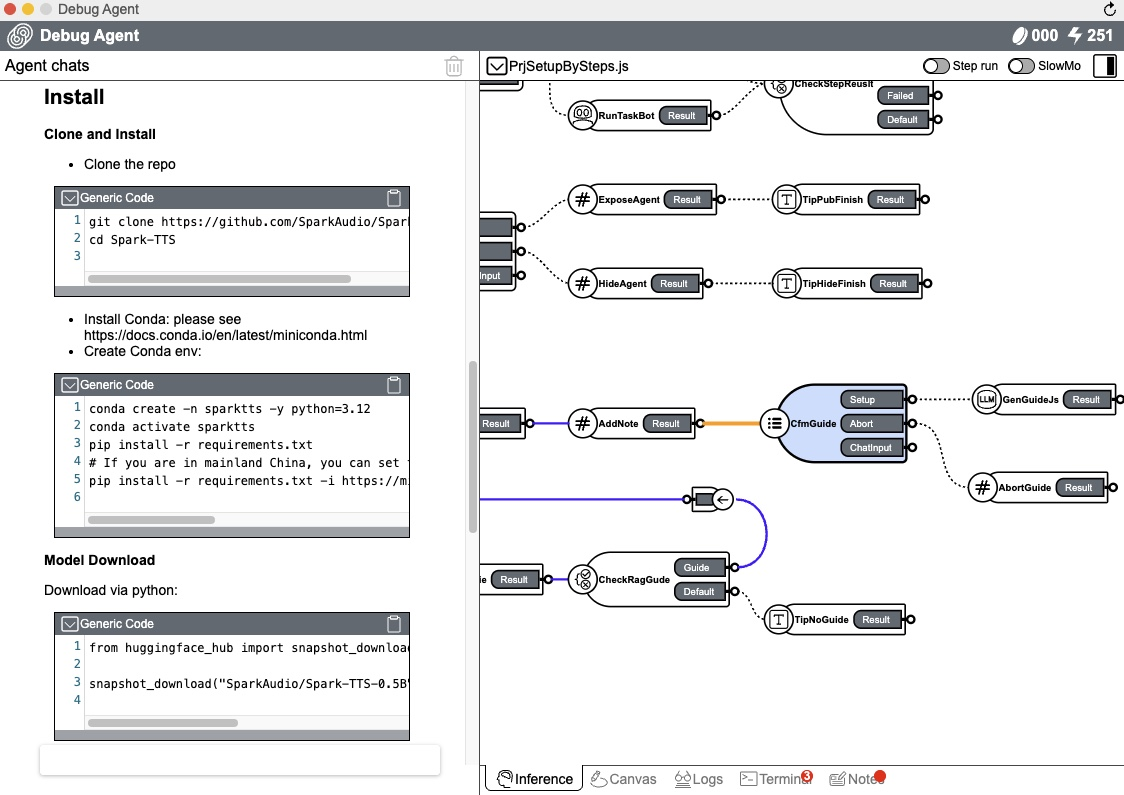
\includegraphics[scale=0.4]{imgs/guidelines_ui_.png}
	\caption{Screenshot of our local auto-deployment process. \textbf{Left:} Execution following predefined guidelines to ensure structured and reliable deployment. \textbf{Right:} The inference and planning interface for dynamically adapting to deployment conditions.}
	\label{fig:guideline}
\end{figure*}

AI2Agent adopts a guideline-driven execution strategy to ensure a structured, efficient, and reliable deployment process. Instead of relying solely on autonomous adjustments, it follows predefined, validated workflows that incorporate best practices and accumulated expertise, as illustrated in Figure~\ref{fig:guideline}.

By adhering to these step-by-step guidelines, AI2Agent minimizes uncertainty and maintains consistency across deployments. In complex or ambiguous scenarios, it proactively references its Knowledge Repository to retrieve relevant cases and proven solutions, thereby reducing unnecessary trial-and-error debugging.

This structured approach not only improves deployment stability and efficiency but also mitigates potential failures by grounding the execution process in historical insights and validated experience.

\subsection{Self-Adaptive Debug}
To address the dynamic nature of deployment environments, AI2Agent integrates a self-adaptive debugging mechanism that refines execution strategies based on real-time feedback. This mechanism consists of three key components:

\paragraph{Step-by-Step Execution} AI2Agent dynamically adjusts its execution flow in response to real-time environmental feedback. During deployment, it continuously monitors system parameters such as computational resources, dependency versions, and runtime errors. Based on this data, AI2Agent adjusts execution parameters to enhance performance and maintain system stability.

\paragraph{Environment-Aware Debug} When deployment failures occur, AI2Agent automatically diagnoses issues by analyzing execution logs and system constraints. It identifies failure patterns, refines its execution strategy, and applies corrective actions to enhance robustness. If necessary, AI2Agent can perform an online search to gather additional information or solutions, further improving its problem-solving capabilities. This proactive approach reduces disruptions and ensures smoother execution.

\paragraph{Knowledge-Guided Refinement} To improve debugging efficiency, AI2Agent queries its Knowledge Repository for relevant failure cases and proven solutions. By leveraging historical insights, AI2Agent accelerates problem resolution and refines debugging techniques, increasing deployment success rates while minimizing human intervention.

\subsection{Case \& Solution Accumulation}
AI2Agent continuously refines its deployment strategies by accumulating experience. The Knowledge Repository serves as a structured database that records successful deployment cases, failure resolutions, and improvement strategies. This module enables two key processes:

\paragraph{Retrieval of Deployment Insights} During deployment, AI2Agent retrieves relevant historical cases using Retrieval-Augmented Generation (RAG). These insights help in selecting optimal configurations, dependency management strategies, and execution plans tailored to the current task.

\paragraph{Continuous Learning and Refinement} Every deployment contributes new insights to the repository. AI2Agent analyzes both successful and failed deployments, extracting lessons from error logs and corrective actions. These insights are integrated into future executions, ensuring a continuously evolving and increasingly autonomous deployment framework.




\begin{algorithm}
%\small
\caption{AI2Agent: Automated AI Deployment}
\label{alg:general_deploy}
\begin{algorithmic}[1]

\Require Repository $R$, Execution Environment $\mathcal{E}$ 
\Return Successfully deployed AI Agent $\mathcal{A}$

\State \textbf{\textcolor{teal}{// Guideline-driven Execution}}  
\State ${G} \gets f_{\text{load}}({R})$  
\State $S \gets \emptyset$ // Store execution results

\For{each step ${G}_t \in {G}$}
    \State \textbf{// Execute step} 
    \State $S_t \gets f_{\text{exec}}(\mathcal{E}, {G}_t)$  
    \State $S \gets S \cup \{S_t\}$  
   \State \textbf{\textcolor{teal}{// Self-adaptive Debug}}  
    \While{$f_{\text{status}}(S_t) = 0$} 
         \State ${G}_t' \gets f_{\text{search}}(S_t,R)$   {//search solutions}
         \State $S_t' \gets f_{\text{exec}}(\mathcal{E}, {G}_t')$  
         \State $S \gets S \cup \{S_t'\}$
     \State \textbf{\textcolor{teal}{// Case \& Solution Accumulation}}
     \State ${R} \gets f_{\text{merge}}({G}_t',S_t')$
    \EndWhile 
\EndFor 

\State \textbf{\textcolor{teal}{// Auto-Deployed AI Agent}}  
\State $\mathcal{A} \gets f_{\text{auto-deploy}}(S)$  
\State \textbf{return} $\mathcal{A}$  

\end{algorithmic}
\end{algorithm}


